\documentclass[11pt,letterpaper]{article}
\usepackage[margin=1in,headheight=15pt]{geometry}
\usepackage[T1]{fontenc}
\usepackage{newpxtext}
\usepackage{microtype}
\usepackage{amsmath,amsthm,mathtools}
\usepackage{newpxmath}
\usepackage{booktabs,array,longtable}
\usepackage{xcolor}
\definecolor{Olive}{HTML}{556343}
\definecolor{PaleOlive}{HTML}{F1F3EC}
\definecolor{WarmGray}{HTML}{66645D}
\definecolor{Salmon}{HTML}{B75F50}
\usepackage{tikz}
\usetikzlibrary{positioning,calc,arrows.meta}
\usepackage[most]{tcolorbox}
\usepackage{enumitem}
\usepackage{fancyhdr}
\usepackage{titlesec}
\usepackage{listings}
\usepackage{hyperref}
\usepackage[nameinlink,noabbrev]{cleveref}
\hypersetup{colorlinks=true,linkcolor=Olive,citecolor=Olive,urlcolor=Olive,
 pdftitle={A marked-cycle proof of the trapezohedral domination conjecture},
 pdfsubject={OEIS A381190: classification, exact enumeration, and limit laws},
 pdfauthor={Research manuscript prepared with ChatGPT}}
\titleformat{\section}{\Large\bfseries\color{Olive}}{\thesection}{0.75em}{}
\titleformat{\subsection}{\large\bfseries\color{Olive}}{\thesubsection}{0.75em}{}
\pagestyle{fancy}
\fancyhf{}
\fancyhead[L]{\small\color{WarmGray}A381190 \quad Marked-cycle enumeration}
\fancyhead[R]{\small\color{WarmGray}19 September 2026}
\fancyfoot[C]{\small\thepage}
\renewcommand{\headrulewidth}{0.3pt}
\setlength{\parskip}{3pt}
\setlength{\parindent}{1.2em}
\setlength{\emergencystretch}{2em}
\linespread{1.035}
\numberwithin{equation}{section}
\newtheorem{theorem}{Theorem}[section]
\newtheorem{lemma}[theorem]{Lemma}
\newtheorem{proposition}[theorem]{Proposition}
\newtheorem{corollary}[theorem]{Corollary}
\theoremstyle{definition}
\newtheorem{definition}[theorem]{Definition}
\newtheorem{example}[theorem]{Example}
\newtheorem{remark}[theorem]{Remark}
\newcommand{\N}{\mathbb N}
\newcommand{\Z}{\mathbb Z}
\newcommand{\C}{\mathbb C}
\newcommand{\E}{\mathbb E}
\newcommand{\Var}{\operatorname{Var}}
\newcommand{\Prob}{\mathbb P}
\newcommand{\CM}{\mathcal D}
\newcommand{\coeff}[2]{[#1^{#2}]}
\newcommand{\dd}{\,\mathrm d}
\newcommand{\1}{\mathbf 1}
\newtcolorbox{resultbox}{colback=PaleOlive,colframe=Olive,boxrule=0.55pt,
 arc=1pt,left=10pt,right=10pt,top=8pt,bottom=8pt}
\lstset{basicstyle=\small\ttfamily,columns=fullflexible,keepspaces=true,
 breaklines=true,frame=single,rulecolor=\color{Olive},backgroundcolor=\color{PaleOlive},
 keywordstyle=\color{Olive}\bfseries,commentstyle=\color{WarmGray},showstringspaces=false}

\begin{document}
\begin{center}
{\small\scshape\color{Olive}An elementary resolution of an OEIS generating-function conjecture}\par
\vspace{13pt}
{\LARGE\bfseries A marked-cycle proof of the\par trapezohedral domination conjecture}\par
\vspace{10pt}
{\large Classification, refined enumeration, log-concavity,\par and asymptotic laws for OEIS A381190}\par
\vspace{12pt}
{\color{WarmGray}Research manuscript prepared for Vladimir\par 19 September 2026}
\end{center}
\vspace{8pt}
\begin{abstract}
Let $a_n$ count vertex subsets of the $n$-trapezohedral graph that are minimal
among all dominating sets and induce a connected subgraph. The OEIS entry
A381190 records a rational generating function conjectured by Joerg Arndt.
We prove this formula by classifying every counted set: it contains exactly
one pole, exactly one vertex of the opposite ring class, and a cyclic binary
word whose zero-to-zero gaps have lengths two or three. The opposite-class
vertex marks an eligible edge of that word. Cutting at the marked gap gives
\[
 a_n=2n\bigl(2p_{n-2}+p_{n-3}\bigr),\qquad
 \sum_{m\ge0}p_mx^m=\frac1{1-x^2-x^3},\qquad n\ge3.
\]
The same bijection gives an explicit size distribution, a trivariate generating
function, strict log-concavity, a distinction between tree and unicyclic
induced subgraphs, exact extremal counts, and an unbiased sampler. We also
obtain a Binet formula, exponentially small absolute asymptotic error, two
exact nearest-integer formulas, a closed finite binomial sum, and a central
limit theorem for set size. Independent exhaustion of all 22,369,536 vertex
subsets for $3\le n\le11$ agrees with the classification at the level of
individual sets, not merely totals; the cases $3\le n\le10$ are independently reproduced by a second, separately written exhaustion, and is reproduced by a second, separately
written exhaustive program in another language.
\end{abstract}

\begin{resultbox}
\textbf{Status and scope.} On 19 September 2026 the live OEIS entry still labels
the generating function as conjectured, with attribution to Joerg Arndt on
7 January 2026 \cite{A381190}. This manuscript supplies a complete
self-contained proof of that assertion. Targeted searches did not locate an
earlier proof; that is not a guarantee of literature priority. The proofs have
been computationally cross-checked, but not formally verified in a proof
assistant or independently peer-reviewed. The OEIS status was checked, but an
exhaustive priority search was not performed; no claim of being the first proof
anywhere in the literature is made. The computational material is independently
reproducible, but is not a formal proof-assistant verification or a substitute
for peer review. No OEIS edit or submission has been made.
\end{resultbox}

\newpage
{\small\setlength{\parskip}{0pt}\tableofcontents}
\newpage

\section{The problem and the answer}\label{sec:problem}

\subsection{The graph and the meaning of minimality}
For $n\ge3$, write $T_n$ for the graph with vertices
\[
 V(T_n)=\{N,S\}\cup\{a_i,b_i:i\in\Z/n\Z\}
\]
and edges
\begin{equation}\label{eq:edges}
 Na_i,\qquad Sb_i,\qquad a_ib_i,\qquad b_ia_{i+1}
 \quad(i\in\Z/n\Z).
\end{equation}
Thus $a_0b_0a_1b_1\cdots a_{n-1}b_{n-1}a_0$ is a ring of length $2n$;
the pole $N$ is joined to every $a_i$ and the pole $S$ to every $b_i$.
This is the usual $n$-trapezohedral graph, with $2n+2$ vertices and $4n$ edges;
$T_3$ is the cube graph \cite{trapezohedral}. All indices below are cyclic.
Sets are counted as subsets of this fixed graph, \emph{not} up to rotation,
reflection, or graph isomorphism.

\begin{definition}
A subset $D\subseteq V(G)$ is \emph{dominating} if every vertex belongs to $D$
or has a neighbor in $D$. It is \emph{minimal dominating} if no proper subset
of $D$ is dominating. We call it a \emph{connected minimal dominating set}
when, in addition, the induced graph $G[D]$ is connected. Let $\CM_n$ denote
this family for $T_n$, and let $a_n=|\CM_n|$.
\end{definition}

The order of these qualifications matters. A \emph{minimal connected dominating
set} is minimal only within the family of connected dominating sets. Such a
set can cease to be connected when one vertex is deleted while remaining
dominating, so it need not be minimal dominating. This distinction is explicit
in the standard definitions \cite{minimal,connectedminimal}. Here every
selected vertex must be indispensable \emph{for domination itself}.

\begin{figure}[ht]
\centering
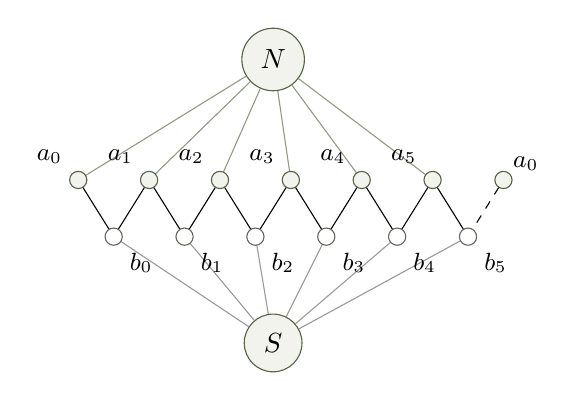
\begin{tikzpicture}[x=0.9cm,y=0.9cm,
 a/.style={circle,draw=Olive,fill=PaleOlive,inner sep=2.2pt},
 b/.style={circle,draw=WarmGray,fill=white,inner sep=2.2pt},
 pole/.style={circle,draw=Olive,fill=PaleOlive,inner sep=4pt}]
\node[pole] (N) at (2.75,2.1) {$N$};
\node[pole] (S) at (2.75,-1.9) {$S$};
\foreach \i in {0,...,5} {
 \coordinate (aa\i) at (\i,0.4);
 \coordinate (bb\i) at (\i+0.5,-0.4);
 \draw[Olive!65] (N)--(aa\i);
 \draw[WarmGray!65] (S)--(bb\i);
 \draw (aa\i)--(bb\i);
}
\foreach \i in {0,...,4} {
 \pgfmathtruncatemacro{\j}{\i+1}
 \draw (bb\i)--(aa\j);
}
\draw[dashed] (bb5)--(6,0.4);
\node[a] at (6,0.4) {};
\node[above right,font=\small] at (6,0.4) {$a_0$};
\foreach \i in {0,...,5} {
 \node[a,label={[font=\small]above left:$a_{\i}$}] at (aa\i) {};
 \node[b,label={[font=\small]below right:$b_{\i}$}] at (bb\i) {};
}
\end{tikzpicture}
\caption{An unrolled drawing of $T_6$. The rightmost $a_0$ repeats the leftmost
vertex; it is not an additional vertex. The repeated boundary makes the ring
and the two alternating pole neighborhoods explicit.}
\label{fig:graph}
\end{figure}

\subsection{The conjecture and a simpler formula}
The entry A381190 was contributed by Eric W. Weisstein on 16 February 2025.
The retrieved entry lists 40 terms, beginning
\[
6,16,30,36,70,96,144,220,308,456,650,924,\ldots
\]
with offset $n=3$, and gives Arndt's conjecture \cite{A381190}
\begin{equation}\label{eq:conjecture}
 \sum_{n\ge3}a_nx^n
 =\frac{-2x^3(4x^5+8x^4+4x^3-9x^2-8x-3)}{(x^3+x^2-1)^2}.
\end{equation}
We will prove the following stronger and more transparent statement.

\begin{theorem}[Main enumeration]\label{thm:main}
Let $p_m$ count ordered compositions of $m$ into parts $2$ and $3$, including
the empty composition when $m=0$. Put $p_m=0$ for $m<0$. Then
\begin{equation}\label{eq:main}
 \boxed{a_n=2n\bigl(2p_{n-2}+p_{n-3}\bigr)\qquad(n\ge3).}
\end{equation}
Equivalently, if $P(m)$ is A000931 with its OEIS indexing, then
\begin{equation}\label{eq:padovan}
 a_n=2n\bigl(2P(n+1)+P(n)\bigr).
\end{equation}
\end{theorem}
The indexing in \eqref{eq:padovan} uses $p_m=P(m+3)$; the composition
interpretation and that shift are recorded in A000931 \cite{A000931}.
The sequence $p_m$ is specified independently by
\begin{equation}\label{eq:p}
 p_0=1,\quad p_1=0,\quad p_2=1,\qquad
 p_m=p_{m-2}+p_{m-3}\quad(m\ge3),
 \qquad \sum_{m\ge0}p_mx^m=\frac1{1-x^2-x^3}.
\end{equation}
The recurrence follows by deleting the first part of a nonempty composition.
Its initial terms are $1,0,1,1,1,2,2,3,4,5,\ldots$.

\section{A structural classification}\label{sec:classification}

\subsection{Private neighbors}
For a vertex $w$, let $N[w]$ denote its closed neighborhood: $w$ together with
all vertices adjacent to $w$.
\begin{lemma}[Private-neighbor criterion]\label{lem:private}
A dominating set $D$ is minimal if and only if every $v\in D$ has a vertex $w$
with
\begin{equation}\label{eq:private}
 N[w]\cap D=\{v\}.
\end{equation}
The vertex $w$ may equal $v$ and is called a private neighbor of $v$ relative to $D$.
\end{lemma}
\begin{proof}
If \eqref{eq:private} holds, deleting $v$ leaves $w$ undominated. Thus no
one-vertex deletion preserves domination, and no proper subset can dominate.
Conversely, if no such $w$ exists for some $v$, every vertex dominated by $v$
is also dominated by another vertex of $D$. Hence $D\setminus\{v\}$ still
dominates, contradicting minimality.
\end{proof}

\subsection{Exactly one pole survives}
\begin{lemma}\label{lem:onepole}
Every $D\in\CM_n$ contains exactly one of $N$ and $S$.
\end{lemma}
\begin{proof}
The pair $\{N,S\}$ dominates $T_n$, so a minimal dominating set containing
both poles must equal that pair. But the poles are not adjacent, and the pair
is disconnected.

Suppose instead that $D$ contains neither pole. Its induced graph lies in the
ring $C_{2n}$. A nonempty connected proper subset of a cycle is a consecutive
path. If this path has $\ell$ vertices, its closed neighborhood within the ring
has at most $\ell+2$ vertices. Because there are no selected poles to dominate
the remaining ring vertices, $\ell\ge2n-2\ge4$. In particular, the path contains
at least two vertices of each alternating class.

Take an internal vertex $v$ of the path. Each of its two ring neighbors belongs
to $D$, so neither $v$ nor either ring neighbor can be private for $v$. Its only
other neighbor is its pole, which is adjacent to at least two selected vertices
of the same class. The pole is not private either. Thus $v$ has no private
neighbor, contradicting \cref{lem:private}. If $D$ is the whole ring, the same
argument applies to every ring vertex.
\end{proof}

By symmetry we may now assume $N\in D$ and $S\notin D$. The explicit symmetry
$N\leftrightarrow S$, $a_i\mapsto b_{-i}$, $b_i\mapsto a_{-i}$ preserves all
edges in \eqref{eq:edges}.

\begin{lemma}\label{lem:oneb}
If $D\in\CM_n$ contains $N$, then it contains exactly one $b$-vertex.
\end{lemma}
\begin{proof}
At least one $b$-vertex is needed to dominate the unselected pole $S$.
Every selected $b_i$ must have a selected $a$-neighbor, since $S$ is absent and
$D$ is connected. Therefore $b_i$ cannot be its own private neighbor.
Neither adjacent $a$-vertex can be private for it, because both are adjacent
to the selected pole $N$. Its only remaining possible private neighbor is $S$.
If two or more $b$-vertices were selected, $S$ would be private for none of them.
Minimality therefore forces exactly one, say $b_j$.
\end{proof}

\subsection{A cyclic word with one marked edge}
Write
\begin{equation}\label{eq:Dword}
 D=\{N,b_j\}\cup\{a_i:x_i=1\},\qquad x_i\in\{0,1\}.
\end{equation}
View $x_0x_1\cdots x_{n-1}$ as a word on the auxiliary cycle with vertices
$a_0,\ldots,a_{n-1}$. Its edge $e_j=(a_j,a_{j+1})$ is distinguished by the
selected vertex $b_j$.

\begin{theorem}[Classification]\label{thm:classification}
The set \eqref{eq:Dword} belongs to $\CM_n$ if and only if the following hold.
\begin{enumerate}[label=\textnormal{(\roman*)},leftmargin=2.4em,itemsep=2pt]
\item The cyclic word contains neither $00$ nor $111$.
\item If the marked edge has endpoints $11$, it is the middle edge of a cyclic
$0110$ pattern.
\item If the marked edge has endpoints $01$ or $10$, its endpoint labeled $1$
is the middle vertex of a cyclic $010$ pattern.
\end{enumerate}
In (ii), the surrounding zeros already follow from (i). A cyclic pattern can
wrap around the end of the word; for $n=3$ the two displayed zeros of $0110$
are the same vertex.
\end{theorem}
\begin{proof}
Every unselected $b_i$ needs a selected $a$-neighbor in order to be dominated.
The selected $b_j$ also needs a selected $a$-neighbor, now for connectivity.
Consequently $x_i+x_{i+1}\ge1$ for every $i$, excluding $00$.

Consider a selected $a_i$. Its closed neighborhood consists of $a_i$, $N$,
$b_{i-1}$, and $b_i$. Neither $a_i$ nor $N$ can be private for $a_i$, because
$N$ is selected. The distinguished $b_j$ is not private for $a_i$, because it
is itself selected. An unselected adjacent $b$-vertex is private for $a_i$
exactly when its other $a$-neighbor is unselected. We obtain the exact rule:
\begin{quote}
Every $1$ must have a neighboring $0$ across an edge other than the marked edge.
\end{quote}
This excludes $111$. If the marker is $11$, each of the two marked endpoints
must find its zero on its other side, giving $0110$. If the marker is $10$ or
$01$, its $1$ must find a second zero on the other side, giving $010$. All other
ones merely need one adjacent zero, which the absence of $111$ ensures.
This proves necessity.

Conversely, suppose the stated word conditions hold. Every $a$-vertex is
dominated by $N$, every $b$-vertex has a selected $a$-neighbor by the absence
of $00$, and $S$ is dominated by $b_j$. All selected $a$-vertices are adjacent
to $N$, while $b_j$ is adjacent to at least one of them, so $D$ is connected.

Every selected $a_i$ has a private neighboring $b$-vertex by the exact rule
above. The vertex $S$ is private for $b_j$. It remains to supply a private
neighbor for $N$. If the marker is $11$, any zero of the word is an unselected
$a$-vertex not incident to the marker; its closed neighborhood meets $D$ only
in $N$. At least one zero exists because $111$ is forbidden and $n\ge3$.
If the marker is $01$ or $10$, use the other zero in the required $010$ pattern.
The two neighbors of its middle vertex are distinct for $n\ge3$, and that
other zero is not incident to the marked edge. Again it is private for $N$.
Thus every selected vertex has a private neighbor, proving minimality.
\end{proof}

\begin{example}[A complete certificate at $n=5$]\label{ex:n5}
Let $n=5$ and take the cyclic word $x_0x_1x_2x_3x_4=01101$ with the marked
edge $e_1=(a_1,a_2)$, so that the selected opposite-class vertex is $b_1$ and
\[
 D=\{N,a_1,a_2,a_4,b_1\}.
\]
The word has no $00$ and no $111$, and the marker has endpoints $11$ sitting
as the middle edge of the cyclic pattern $x_0x_1x_2x_3=0110$; conditions
(i) and (ii) of \cref{thm:classification} therefore hold. A complete
private-neighbor certificate is
\begin{center}
\begin{tabular}{l@{\qquad}ccccc}
\toprule
Selected vertex & $N$ & $a_1$ & $a_2$ & $a_4$ & $b_1$\\
Private neighbor & $a_0$ & $b_0$ & $b_2$ & $b_3$ & $S$\\
\bottomrule
\end{tabular}
\end{center}
Each column is checked directly from \eqref{eq:edges}. For instance
$N[a_0]=\{a_0,N,b_4,b_0\}$ meets $D$ only in $N$, and
$N[b_0]=\{b_0,S,a_0,a_1\}$ meets $D$ only in $a_1$; the pole $S$ is adjacent
to $b_1$ alone among the selected vertices. The zero set is $Y=\{0,3\}$, so
$k=2$ with one gap of each length, and \eqref{eq:eligiblecount} predicts
$4k-n=3$ eligible markers. Counting the five labeled rotations, the three
markers, and the two poles gives $a_5=2\cdot5\cdot3=30$, in agreement with
\eqref{eq:sizecount} below.
\end{example}

The archived file \texttt{data/certificates\_n5.json} lists all thirty members
of $\CM_5$ together with such a witness for every selected vertex. That file
and the standard-library verifier that produced it use the one-based labels
$u,v,a_1,\dots,a_n,b_1,\dots,b_n$ of the incoming package
(\cref{sec:provenance}); the dictionary to the labels used here is
$u=N$, $v=S$, $a_i=a_{i-1}$, $b_i=b_{i-1}$. Under it, the certificate above
is the row $D=\{u,a_2,a_3,a_5,b_2\}$ of that file.

\subsection{The gap formulation}
Let $Y=\{i:x_i=0\}$. The absence of $00$ means that $Y$ is independent in
$C_n$; the absence of $111$ means that every vertex outside $Y$ is adjacent
to $Y$. Thus $Y$ is a \emph{maximal independent set} of $C_n$. In the cyclic
order, distances between consecutive zeros are exactly $2$ or $3$.
These are the two possible blocks $01$ and $011$, with the next block starting
at the next zero.

\begin{corollary}[Marked gaps]\label{cor:gaps}
In a zero-to-zero gap of length $2$, both edges are eligible markers.
In a gap of length $3$, only the middle edge is eligible.
There are no other possibilities.
\end{corollary}

\begin{figure}[ht]
\centering
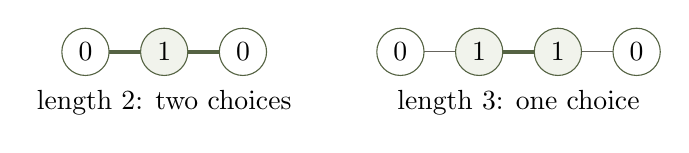
\begin{tikzpicture}[x=1cm,y=1cm,
 zero/.style={circle,draw=Olive,fill=white,minimum size=6mm,inner sep=0pt},
 one/.style={circle,draw=Olive,fill=PaleOlive,minimum size=6mm,inner sep=0pt}]
\draw[Olive,line width=1.6pt] (0,0)--(1,0)--(2,0);
\node[zero] at (0,0) {$0$}; \node[one] at (1,0) {$1$};
\node[zero] at (2,0) {$0$};
\node at (1,-0.65) {length $2$: two choices};
\draw[WarmGray] (4,0)--(5,0); \draw[WarmGray] (6,0)--(7,0);
\draw[Olive,line width=1.6pt] (5,0)--(6,0);
\node[zero] at (4,0) {$0$}; \node[one] at (5,0) {$1$};
\node[one] at (6,0) {$1$}; \node[zero] at (7,0) {$0$};
\node at (5.5,-0.65) {length $3$: one choice};
\end{tikzpicture}
\caption{Eligible marked edges are thick. Adjacent gaps share their endpoint
zero. When there is only one gap, its two displayed endpoint zeros coincide
on the cycle.}
\label{fig:gaps}
\end{figure}
The unmarked objects are classical: maximal independent sets of $C_n$ are
counted by the Perrin numbers \cite{A001608}. The essential step here is the
precise edge-marking condition imposed by private neighbors in $T_n$.

\section{Cutting at the marker: proof of the conjecture}\label{sec:proofgf}

\subsection{The rooted composition bijection}
Fix the selected pole $N$ and the selected opposite-class vertex $b_0$.
There are three possible local marker configurations.
If the marked edge is $11$, it sits inside one length-$3$ gap. Remove that
anchored gap and read the remaining gaps in the fixed cyclic orientation.
They form an ordered composition of $n-3$ into $2$'s and $3$'s, and the operation
is reversible. Hence there are $p_{n-3}$ such words.

If the marker has type $01$, it is one of the two edges of a length-$2$ gap.
Removing that anchored gap leaves a composition of $n-2$. The same is true
for type $10$, but its orientation relative to the fixed marker is different.
These cases are disjoint and contribute $2p_{n-2}$.

This argument includes the empty remainder. In particular, for $n=3$ the
length-$3$ gap can occupy the whole cycle, contributing $p_0=1$ for a fixed
pole and marker. The length-$2$ alternatives contribute $p_1=0$.

There are two choices of the selected pole and $n$ choices of its unique
opposite-class vertex. These choices are recoverable from $D$, so they cannot
create overcounting. This proves \cref{thm:main}.

The same bijection can be read blockwise instead of gapwise: starting at the
initial zero of the marked gap and reading in the fixed cyclic orientation
produces a \emph{marked first block} --- a block $01$ carrying either of its two
marks, or a block $011$ carrying its unique mark, which is exactly the
numerator $2x^2+x^3$ of \eqref{eq:R} below --- followed by a free ordered list
of unmarked blocks, which is exactly the factor $1/(1-x^2-x^3)$. In either
reading the mark singles out one specific block, so a periodic word creates no
rotational ambiguity and no division by an orbit size is needed.

\subsection{The generating function}
Introduce
\begin{equation}\label{eq:R}
 R(x)=\frac{2x^2+x^3}{1-x^2-x^3}.
\end{equation}
For $n\ge3$, its $x^n$ coefficient is $a_n/(2n)$. There is also an artificial
$x^2$ coefficient equal to $2$; no graph with $n=2$ is included in this problem.
Since $x\frac{\mathrm d}{\mathrm dx}$ multiplies the $x^n$ coefficient by $n$,
\begin{align}\label{eq:derivativegf}
 A(x):=\sum_{n\ge3}a_nx^n
 &=2xR'(x)-8x^2\\
 &=\frac{-2x^3(4x^5+8x^4+4x^3-9x^2-8x-3)}{(x^3+x^2-1)^2}.\notag
\end{align}
This is exactly \eqref{eq:conjecture}. The squared denominator is explained
structurally: after fixing a pole, an eligible location is marked on a cyclic
object, introducing a factor of $n$ into a Padovan-type count.

\begin{table}[ht]
\centering
\begin{tabular}{rrrrr}
\toprule
$n$ & $p_{n-2}$ & $p_{n-3}$ & $a_n/(2n)$ & $a_n$\\
\midrule
3&0&1&1&6\\
4&1&0&2&16\\
5&1&1&3&30\\
6&1&1&3&36\\
7&2&1&5&70\\
8&2&2&6&96\\
9&3&2&8&144\\
10&4&3&11&220\\
11&5&4&14&308\\
12&7&5&19&456\\
13&9&7&25&650\\
14&12&9&33&924\\
\bottomrule
\end{tabular}
\caption{Initial values computed from the bijection. These agree with the
corresponding published A381190 terms \cite{A381190}.}
\end{table}

\section{Exact size and topology refinements}\label{sec:refined}

\subsection{Counting fixed gap multiplicities}
Let $k=|Y|$ be the number of zeros, let $s$ be the number of length-$2$ gaps,
and let $t$ be the number of length-$3$ gaps. Then
\begin{equation}\label{eq:st}
 s+t=k,\qquad 2s+3t=n,\qquad s=3k-n,\qquad t=n-2k.
\end{equation}
Consequently
\begin{equation}\label{eq:krange}
 \left\lceil\frac n3\right\rceil\le k\le
 \left\lfloor\frac n2\right\rfloor,
 \qquad |D|=n-k+2.
\end{equation}

The number of labeled cyclic zero sets with these multiplicities is
\begin{equation}\label{eq:cycliccount}
 \frac nk\binom{k}{t}.
\end{equation}
Indeed, distinguish a zero and select its index in $n$ ways; choose the
positions of the $t$ long gaps among the $k$ ordered gaps in $\binom{k}{t}$
ways. This counts each unrooted zero set exactly $k$ times, once per choice
of its distinguished zero. The reasoning is valid even when the gap word is
periodic: the root is an actual labeled cycle vertex, not a necklace orbit.

By \cref{cor:gaps}, a zero set has
\begin{equation}\label{eq:eligiblecount}
 2s+t=4k-n
\end{equation}
eligible markers. This number depends only on $n$ and $k$.

\begin{theorem}[The complete size distribution]\label{thm:size}
For $k$ in \eqref{eq:krange}, the number $c_{n,k}$ of sets in $\CM_n$ of
cardinality $n-k+2$ is
\begin{align}\label{eq:sizecount}
 c_{n,k}
 &=\frac{2n(4k-n)}{k}\binom{k}{n-2k}\\
 &=2n\left(2\binom{k-1}{n-2k}+\binom{k-1}{n-2k-1}\right).\notag
\end{align}
Outside that range, the count is zero. A binomial coefficient is interpreted
as zero when its lower index is negative or exceeds its nonnegative upper index.
\end{theorem}
\begin{proof}
Multiply \eqref{eq:cycliccount} by the eligible-marker count
\eqref{eq:eligiblecount} and by the two choices of pole. For the second form,
use $(s/k)\binom{k}{t}=\binom{k-1}{t}$ and
$(t/k)\binom{k}{t}=\binom{k-1}{t-1}$, with $2s+t=4k-n$.
\end{proof}

Summing \cref{thm:size} over the admissible sizes turns the Padovan recurrence
of \cref{thm:main} into a closed finite sum, with no recurrence and no
generating function.

\begin{corollary}[A finite binomial sum for the total]\label{cor:finitesum}
For every $n\ge3$, with $s$ and $t$ the numbers of length-$2$ and length-$3$
gaps as in \eqref{eq:st},
\begin{equation}\label{eq:finitesum}
 a_n=2n\!\!\sum_{\substack{s,t\ge0\\2s+3t=n}}\!\!
 \left(2\binom{s+t-1}{t}+\binom{s+t-1}{t-1}\right)
 =2n\!\!\sum_{\substack{s,t\ge0\\2s+3t=n}}\!\!
 \frac{2s+t}{s+t}\binom{s+t}{t}.
\end{equation}
\end{corollary}
\begin{proof}
Each pair $(s,t)$ with $2s+3t=n$ corresponds to the single admissible
$k=s+t$ of \eqref{eq:st}, and the summand is $c_{n,k}/(2n)$ in the two forms
of \eqref{eq:sizecount}. Summing over $k$ gives $a_n$. The two summands agree
term by term because, writing $k=s+t$ and $s=k-t$,
\begin{equation}\label{eq:binomid}
 2\binom{k-1}{t}+\binom{k-1}{t-1}
 =\frac{2(k-t)+t}{k}\binom{k}{t}
 =\frac{2s+t}{k}\binom{k}{t}.
\end{equation}
\end{proof}
Although the second form of \eqref{eq:finitesum} displays a quotient, every
summand of the first form is visibly a nonnegative integer. This gives a direct
combinatorial reason, independent of \eqref{eq:divisibility} below, that
$a_n/(2n)$ is an integer: it is the number of completions once one pole and one
marker block have been fixed.

\subsection{Only two induced graph shapes occur}
In \eqref{eq:Dword}, the pole $N$ is joined to all $n-k$ selected $a$-vertices.
The vertex $b_j$ is joined to either one or two of them, depending on its marker.
There are no other edges in the induced graph.

\begin{corollary}[Trees and four-cycles]\label{cor:topology}
Every member of $\CM_n$ induces either a tree or a unicyclic graph whose unique
cycle has length $4$. For $t=n-2k$, their respective counts at size $n-k+2$ are
\begin{equation}\label{eq:topologyrefined}
 T_{n,k}=4n\binom{k-1}{t},\qquad
 U_{n,k}=2n\binom{k-1}{t-1}.
\end{equation}
In total,
\begin{equation}\label{eq:topologytotal}
 T_n=4n p_{n-2},\qquad U_n=2n p_{n-3},\qquad a_n=T_n+U_n.
\end{equation}
\end{corollary}
\begin{proof}
A marker $01$ or $10$ attaches $b_j$ as a leaf to one leaf of the pole-centered
star. A marker $11$ adds the path $a_jb_ja_{j+1}$ between two leaves and hence
creates precisely the cycle $Na_jb_ja_{j+1}N$. A fixed zero set has $2s$ tree
markers and $t$ unicyclic markers. Multiplying as before proves
\eqref{eq:topologyrefined}; the rooted-composition bijection proves
\eqref{eq:topologytotal} directly.
\end{proof}

\begin{figure}[ht]
\centering
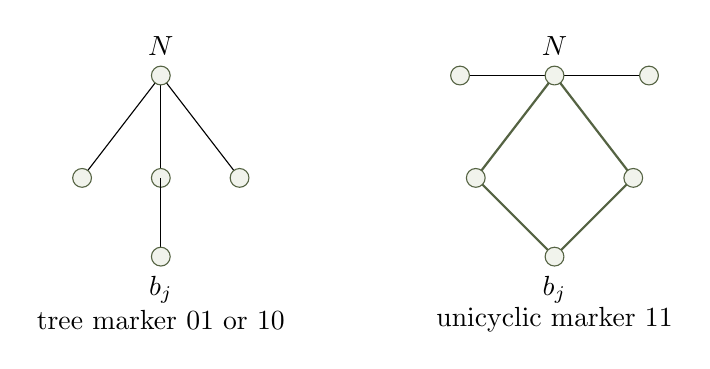
\begin{tikzpicture}[x=1cm,y=1cm,
 vert/.style={circle,draw=Olive,fill=PaleOlive,inner sep=2.4pt}]
\coordinate (N) at (0,1.3);
\foreach \p in {(-1,0),(0,0),(1,0)} {\draw (N)--\p; \node[vert] at \p {};}
\draw (0,0)--(0,-1); \node[vert,label=below:$b_j$] at (0,-1) {};
\node[vert,label=above:$N$] at (N) {};
\node at (0,-1.8) {tree marker $01$ or $10$};
\coordinate (M) at (5,1.3);
\draw[Olive,thick] (M)--(4,0)--(5,-1)--(6,0)--(M);
\draw (M)--(3.8,1.3); \draw (M)--(6.2,1.3);
\foreach \p in {(4,0),(6,0),(3.8,1.3),(6.2,1.3)} {\node[vert] at \p {};}
\node[vert,label=above:$N$] at (M) {};
\node[vert,label=below:$b_j$] at (5,-1) {};
\node at (5,-1.8) {unicyclic marker $11$};
\end{tikzpicture}
\caption{Representative induced shapes. More selected $a$-vertices simply add
leaves adjacent to the pole; no further cycles can arise.}
\end{figure}

\subsection{A trivariate generating function}
Let $y$ mark the size of $D$, and let $v$ mark the unicyclic type. Define
\begin{equation}\label{eq:Fdef}
 f_n(y,v)=\sum_{D\in\CM_n}y^{|D|}v^{\1\{T_n[D]\text{ unicyclic}\}},
 \qquad F(x,y,v)=\sum_{n\ge3}f_n(y,v)x^n.
\end{equation}
A length-$2$ gap contains one selected $a$-vertex and has weight $yx^2$.
A length-$3$ gap contains two and has weight $y^2x^3$. The chosen pole and
opposite-class vertex contribute another factor $y^2$.
The marker belongs either to a length-$2$ gap, with two orientations, or to a
length-$3$ gap, with one unicyclic orientation. Thus
\begin{theorem}[Joint generating function]\label{thm:trivariate}
\begin{equation}\label{eq:trivariate}
 \boxed{F(x,y,v)=2y^2x\frac{\partial}{\partial x}
 \left(\frac{2yx^2+v y^2x^3}{1-yx^2-y^2x^3}\right)-8y^3x^2.}
\end{equation}
\end{theorem}
The derivative accounts for the $n$ possible markers, the outer $2$ for the
pole, and the last term removes the artificial $n=2$ contribution.
Writing $f_n(y)=f_n(y,1)$, the first examples are
\begin{align*}
 f_3(y)&=6y^4,& f_4(y)&=16y^4,& f_5(y)&=30y^5,\\
 f_6(y)&=24y^5+12y^6,& f_7(y)&=70y^6,&
 f_8(y)&=32y^6+64y^7.
\end{align*}
The unexpanded derivative form of \eqref{eq:trivariate} retains the combinatorial
meaning more clearly than its expanded rational numerator. For symbolic use,
however, the size-refined specialization does have a compact closed form.

\begin{corollary}[Expanded size-refined generating function]\label{cor:bivariate}
Carrying out the differentiation in \eqref{eq:trivariate} at $v=1$ gives
\begin{equation}\label{eq:bivariate}
 F(x,y,1)=\sum_{n\ge3}f_n(y)x^n
 =\frac{-2x^3y^4\bigl(4x^5y^3+8x^4y^2+4x^3y-9x^2y-8x-3\bigr)}
        {(x^3y^2+x^2y-1)^2}.
\end{equation}
Setting $y=1$ recovers \eqref{eq:conjecture}.
\end{corollary}
The substitution $x\mapsto x$, $y\mapsto1$ sends the denominator
$(x^3y^2+x^2y-1)^2$ to $(x^3+x^2-1)^2$ and the numerator to that of
\eqref{eq:conjecture}, so \eqref{eq:bivariate} is a genuine refinement of the
conjectured formula rather than a separate claim. It is the convenient form for
automatic coefficient extraction; \eqref{eq:trivariate} is the convenient form
for reading off the combinatorics.

\subsection{A weighted Perrin identity}
Let
\[
 I_n(z)=\sum_{Y\text{ maximal independent in }C_n}z^{|Y|}.
\]
From the rooted-gap count \eqref{eq:cycliccount},
\begin{align}\label{eq:perringf}
 H(x,z):=\sum_{n\ge3}I_n(z)x^n
 &=x\frac{\partial}{\partial x}\sum_{k\ge1}
       \frac{(zx^2+zx^3)^k}{k}-2zx^2\\
 &=\frac{2zx^2+3zx^3}{1-zx^2-zx^3}-2zx^2.\notag
\end{align}
Because a zero set with $k$ vertices contributes $2(4k-n)$ marked objects,
\begin{equation}\label{eq:perrinweighted}
 a_n=2\bigl(4I_n'(1)-nI_n(1)\bigr),\qquad
 A(x)=\left.(8z\partial_z-2x\partial_x)H(x,z)\right|_{z=1}.
\end{equation}
At $z=1$, $I_n(1)$ is the usual Perrin cycle count \cite{A001608}.
The new enumeration is therefore a specific weighted first moment of that
classical family, not an unrelated recurrence coincidence.

\section{Recurrences and exact extremal information}\label{sec:recurrences}

\subsection{A third-order recurrence after normalization}
Let $b_n=a_n/(2n)$ for $n\ge3$. By \eqref{eq:main},
\begin{equation}\label{eq:bnrec}
 b_3=1,\quad b_4=2,\quad b_5=3,\qquad
 b_n=b_{n-2}+b_{n-3}\quad(n\ge6).
\end{equation}
Equivalently,
\begin{equation}\label{eq:anpolyrec}
 (n-2)(n-3)a_n
 =n(n-3)a_{n-2}+n(n-2)a_{n-3}\quad(n\ge6).
\end{equation}
The size polynomials satisfy the parallel recurrence
\begin{equation}\label{eq:fnrec}
 \frac{f_n(y)}n
 =y\frac{f_{n-2}(y)}{n-2}
  +y^2\frac{f_{n-3}(y)}{n-3}\quad(n\ge6).
\end{equation}
The same equation holds with $f_n(y,v)$ in place of $f_n(y)$.
These formulas follow by multiplying the normalized generating function by
$1-yx^2-y^2x^3$, or by deleting the first unmarked gap.

Without normalization, the constant-coefficient recurrence is
\begin{equation}\label{eq:anrec}
 a_n=2a_{n-2}+2a_{n-3}-a_{n-4}-2a_{n-5}-a_{n-6}
 \quad(n\ge9).
\end{equation}
The starting index $9$ is essential: the numerator in \eqref{eq:conjecture}
has degree $8$. The six initial values are
$a_3=6,a_4=16,a_5=30,a_6=36,a_7=70,a_8=96$.

In fact, order $6$ is the minimal order of an eventual constant-coefficient
homogeneous recurrence. Write $Q(x)=1-x^2-x^3$ and $\Pi(x)=2x^2+x^3=x^2(2+x)$,
so that $R=\Pi/Q$ in \eqref{eq:R}. Each step is a concrete evaluation.
\begin{itemize}[leftmargin=1.6em,itemsep=1pt]
\item The roots of $Q$ are simple. Indeed $Q'(x)=-x(2+3x)$ vanishes only at
 $x=0$ and $x=-2/3$, while $Q(0)=1$ and $Q(-2/3)=23/27$ are both nonzero, so
 $Q$ and $Q'$ have no common root.
\item $\Pi$ and $Q$ have no common root. The roots of $\Pi$ are $0$ and $-2$,
 while $Q(0)=1$ and $Q(-2)=5$.
\item At a root $x_0$ of $Q$ the numerator $2x(\Pi'Q-\Pi Q')$ of $2xR'$ takes
 the value $-2x_0\Pi(x_0)Q'(x_0)$, which is nonzero by the two preceding points and
 $x_0\ne0$. Hence $2xR'$ has a genuine double pole at each of the three roots,
 and subtracting the polynomial $8x^2$ cannot remove it.
\end{itemize}
Thus the reduced denominator of $A$ is $Q^2$, of degree $6$. An eventual
constant-coefficient recurrence with characteristic polynomial $\Phi$ makes
$\Phi(x)A(x)$ a polynomial, so $Q^2$ divides $\Phi$ and $\deg\Phi\ge6$; no
lower-order recurrence can suffice. This is a statement about \emph{constant}
coefficients only, and does not conflict with the three-term
polynomial-coefficient recurrence \eqref{eq:anpolyrec}.

The factor $2n$ in \eqref{eq:sizecount} proves the stronger divisibility
\begin{equation}\label{eq:divisibility}
 2n\mid c_{n,k},\qquad 2n\mid T_{n,k},\qquad 2n\mid U_{n,k}.
\end{equation}
Fixing the pole and marker also explains this divisibility combinatorially:
all $2n$ such choices have the same number of completions at each size and type.

\subsection{Smallest and largest possible sets}
\begin{theorem}[Extremal sizes and their multiplicities]\label{thm:extrema}
Every integer size in the interval
\begin{equation}\label{eq:sizerange}
 \left\lceil\frac n2\right\rceil+2
 \ \le |D|\le\left\lfloor\frac{2n}3\right\rfloor+2
\end{equation}
occurs in $\CM_n$. The number of sets attaining the lower endpoint is
\begin{equation}\label{eq:mincounts}
 \begin{cases}
 4n,&n\text{ even},\\
 2n(n-2),&n\text{ odd}.
 \end{cases}
\end{equation}
For the upper endpoint, writing $n=3m+r$ with $r\in\{0,1,2\}$, the count is
\begin{equation}\label{eq:maxcounts}
 \begin{cases}
 2n,&r=0,\\
 nm(m+3),&r=1,\\
 2n(m+2),&r=2.
 \end{cases}
\end{equation}
\end{theorem}
\begin{proof}
The admissible $k$ in \eqref{eq:krange} are consecutive and each has $s,t\ge0$,
so a corresponding gap word exists. Its marker count $2s+t$ is positive.
Since $|D|=n-k+2$, this proves \eqref{eq:sizerange} and attainment.
For the smallest size use $k=\lfloor n/2\rfloor$: $t=0$ for even $n$, and
$t=1$ for odd $n$. Substitution in \eqref{eq:sizecount} gives
\eqref{eq:mincounts}. For the largest size use $k=\lceil n/3\rceil$.
When $n=3m,3m+1,3m+2$, the pairs $(s,t)$ are respectively
$(0,m),(2,m-1),(1,m)$. The same formula simplifies to
\eqref{eq:maxcounts}.
\end{proof}

\subsection{A growing gap between two notions of minimality}
Let $\gamma_c(T_n)$ be the ordinary connected domination number: the minimum
size of any connected dominating set, without requiring minimal domination.
\begin{proposition}\label{prop:gammac}
For every $n\ge3$, $\gamma_c(T_n)=4$, whereas the smallest connected minimal
dominating set has size $\lceil n/2\rceil+2$.
\end{proposition}
\begin{proof}
The set $\{N,a_0,b_0,S\}$ is connected and dominating, proving the upper bound $4$.
A connected dominating set containing both poles needs at least two ring
vertices to connect them, since their distance is $3$. If it contains neither
pole and has at most three vertices, it is a ring path and dominates at most
five ring vertices, fewer than $2n$. If it contains exactly one pole, say $N$,
and has at most three vertices, it needs a selected $b$-vertex to dominate $S$
and a selected $a$-vertex to connect that $b$ to $N$. Thus it consists of $N$
and one adjacent $a,b$ pair. The selected $a$ dominates only its two adjacent
$b$-vertices, one of which is the selected $b$ itself; a third $b$-vertex is
undominated. Hence no such set exists. The second assertion is
\cref{thm:extrema}.
\end{proof}
Thus confusing the two families would not produce a harmless constant-factor
error: their smallest cardinalities separate linearly with $n$.

\section{Strict log-concavity of the size distribution}\label{sec:logconcavity}

\begin{theorem}\label{thm:logconcavity}
For fixed $n$, the positive sequence $(c_{n,k})$ on the interval
\eqref{eq:krange} is strictly log-concave at every interior index:
\begin{equation}\label{eq:logconcavity}
 c_{n,k}^2>c_{n,k-1}c_{n,k+1}.
\end{equation}
The same is true for the nonzero coefficients of $f_n(y)$, read in increasing
size. In particular the distribution is unimodal, with either one mode or
two adjacent equal modes. If the support has at most two points, the strict
log-concavity assertion has no interior inequality to check.
\end{theorem}
\begin{proof}
For two consecutive admissible indices, direct cancellation in
\eqref{eq:sizecount} gives
\begin{align}\label{eq:ratio}
 \frac{c_{n,k+1}}{c_{n,k}}
 &=\frac{4k+4-n}{4k-n}
   \frac{k(n-2k)(n-2k-1)}
   {(3k-n+1)(3k-n+2)(3k-n+3)}\\
 &=\left(1+\frac4{4k-n}\right)
   \frac{k}{3k-n+3}
   \frac{n-2k}{3k-n+1}
   \frac{n-2k-1}{3k-n+2}.\notag
\end{align}
Every displayed factor is positive on the transition interval. The first is
strictly decreasing. The second has derivative
$(3-n)/(3k-n+3)^2\le0$. The third and fourth are strictly decreasing because
their numerators decrease and their positive denominators increase.
Thus the ratio in \eqref{eq:ratio} strictly decreases with $k$ whenever two
successive ratios are defined. This is exactly strict log-concavity.
Replacing $k$ by the reversed index $|D|=n-k+2$ preserves the inequalities.
Decreasing positive consecutive ratios can cross $1$ only once, giving the
stated description of the modes.
\end{proof}
This result is an exact finite-$n$ statement. It is stronger than the visual
bell shape suggested by the asymptotic normal law proved below and does not
rely on that approximation.

\section{Binet formula, asymptotics, and exact rounding}\label{sec:asymptotic}

\subsection{Three characteristic roots}
Let $\alpha$ be the positive real root of
\begin{equation}\label{eq:plastic}
 \alpha^3=\alpha+1,
 \qquad\alpha=1.324717957244746025960908854478\ldots,
\end{equation}
and let $\beta,\overline\beta$ be the other two roots. The polynomial
$z^3-z-1$ has three distinct roots and exactly one real root: at its two real
critical points the polynomial is negative, while it tends to opposite
infinities at the two ends of the real line. By Vieta's formulas,
\begin{equation}\label{eq:betas}
 \beta+\overline\beta=-\alpha,\qquad
 \beta\overline\beta=\alpha^{-1},\qquad
 |\beta|=\alpha^{-1/2}<1.
\end{equation}
Write
\begin{equation}\label{eq:C}
 C(z)=\frac{2z+1}{2z+3},\qquad
 K=2C(\alpha)=1.291964709301166107055203050684\ldots.
\end{equation}

\begin{theorem}[Exact Binet formula]\label{thm:binet}
For every $n\ge3$,
\begin{equation}\label{eq:binet}
 a_n=2n\left(C(\alpha)\alpha^n+C(\beta)\beta^n+
                 C(\overline\beta)\overline\beta^{\,n}\right).
\end{equation}
Consequently
\begin{equation}\label{eq:asymptotic}
 a_n=Kn\alpha^n+O\bigl(n\alpha^{-n/2}\bigr),
\end{equation}
and, more explicitly,
\begin{equation}\label{eq:error}
 |a_n-Kn\alpha^n|\le4n|C(\beta)|\alpha^{-n/2},
 \qquad |C(\beta)|=0.580110540477999273668313348466\ldots.
\end{equation}
\end{theorem}
\begin{proof}
At a pole $x=1/\lambda$ of $R(x)$, where $\lambda^3=\lambda+1$, the coefficient
of $(1-\lambda x)^{-1}$ in its partial fraction decomposition is
\[
 \frac{2+1/\lambda}{2+3/\lambda}=C(\lambda).
\]
Because numerator and denominator of $R$ have equal degree, there is also the
constant polynomial part $-1$. Hence
\begin{equation}\label{eq:partialfraction}
 R(x)=-1+\sum_{\lambda\in\{\alpha,\beta,\overline\beta\}}
                \frac{C(\lambda)}{1-\lambda x}.
\end{equation}
For positive coefficient indices the constant is irrelevant. Extracting the
$x^n$ coefficient and using \eqref{eq:main} proves \eqref{eq:binet}.
The conjugate pair and \eqref{eq:betas} give \eqref{eq:error} by the triangle
inequality, and then \eqref{eq:asymptotic} follows.
\end{proof}

The error here tends to zero \emph{absolutely}, despite the exponential growth
of $a_n$. Relative to the main term it is $O(\alpha^{-3n/2})$.
There is no hidden series of inverse powers of $n$: the entire dominant
contribution is exactly $Kn\alpha^n$, and the remainder consists of the two
explicit, exponentially decaying oscillatory terms in \eqref{eq:binet}.

\subsection{An exact nearest-integer formula}
\begin{theorem}\label{thm:rounding}
For all $n\ge4$,
\begin{equation}\label{eq:rounding}
 \boxed{a_n=2n\left\lfloor C(\alpha)\alpha^n+\frac12\right\rfloor.}
\end{equation}
The exceptional value is $a_3=6$; the same rounding expression at $n=3$
would give $12$.
\end{theorem}
\begin{proof}
For $b_n=a_n/(2n)$, \eqref{eq:binet} gives
\[
 |b_n-C(\alpha)\alpha^n|\le2|C(\beta)|\alpha^{-n/2}.
\]
The bound decreases with $n$, and it is already less than $1/2$ at $n=6$.
Here is an exact certificate, rather than a numerical assumption. From
\eqref{eq:betas},
\[
 |C(\beta)|^2=
 \frac{4-2\alpha^2+\alpha}{4-6\alpha^2+9\alpha}.
\]
The desired inequality at $n=6$ is
$16|C(\beta)|^2<\alpha^6$. Reducing its numerator with
$\alpha^3=\alpha+1$ leaves
\[
 42\alpha^2-8\alpha-63>0.
\]
The rational interval
$13247/10000<\alpha<13248/10000$ is certified by the signs of
$z^3-z-1$ at its endpoints and monotonicity for $z>1$. The last quadratic is
increasing on this interval, and at its lower endpoint it is exactly
$5263189/50000000>0$. The denominator above is positive on the same interval.
This proves the bound for every $n\ge6$.

The remaining cases follow by rational interval substitution in the increasing
function $C(z)z^n$ for $z>1$:
\[
 1.98<C(\alpha)\alpha^4<2.00,\qquad
 2.63<C(\alpha)\alpha^5<2.64.
\]
Their nearest integers are $b_4=2$ and $b_5=3$. Finally,
$1.50<C(\alpha)\alpha^3<1.51$, whose nearest integer is $2$, whereas $b_3=1$.
\end{proof}

\Cref{thm:rounding} rounds the \emph{normalized} count $b_n=a_n/(2n)$.
One can also round $a_n$ itself, at the cost of a much later threshold.

\begin{corollary}[Rounding the unnormalized count]\label{cor:roundingraw}
For every integer $n\ge45$,
\begin{equation}\label{eq:roundingraw}
 a_n=\left\lfloor Kn\alpha^n+\frac12\right\rfloor,
 \qquad K=2C(\alpha).
\end{equation}
The threshold $45$ is sufficient; no minimality claim is made for it.
\end{corollary}
\begin{proof}
First, $|C(\beta)|<1$, by an exact comparison rather than by its decimal value.
With the expression for $|C(\beta)|^2$ displayed in the proof of
\cref{thm:rounding}, the denominator $4-6\alpha^2+9\alpha$ exceeds the
numerator $4-2\alpha^2+\alpha$ by $4\alpha(2-\alpha)>0$, and the denominator is
positive on the certified interval $13247/10000<\alpha<13248/10000$.
Hence \eqref{eq:error} weakens to
\begin{equation}\label{eq:crudeerror}
 |a_n-Kn\alpha^n|<4n\alpha^{-n/2}.
\end{equation}
Next, $\alpha>64/49$. The function $t^3-t-1$ is increasing for $t>1$, and
\[
 \left(\frac{64}{49}\right)^{3}-\frac{64}{49}-1=-\frac{9169}{117649}<0,
\]
so the real root lies above $64/49$. Therefore $\alpha^{-1/2}<7/8$ and
\eqref{eq:crudeerror} gives $|a_n-Kn\alpha^n|<4n(7/8)^n$. The right-hand side
decreases for integer $n\ge8$, since $\frac{n+1}{n}\cdot\frac78<1$ exactly when
$n>7$. At $n=45$ the inequality $4\cdot45\cdot7^{45}<\tfrac12\cdot8^{45}$ is the
integer statement
\begin{equation}\label{eq:integercertificate}
 360\cdot7^{45}<8^{45},
\end{equation}
which holds. Hence the error is strictly below $1/2$ for every $n\ge45$, and
since $a_n$ is an integer, \eqref{eq:roundingraw} follows.
\end{proof}

\begin{remark}\label{rem:twothresholds}
\Cref{thm:rounding} and \cref{cor:roundingraw} round \emph{different}
quantities, and neither threshold corrects the other. The normalized error
$|b_n-C(\alpha)\alpha^n|\le2|C(\beta)|\alpha^{-n/2}$ carries no factor of $n$
and falls below $1/2$ already at $n=6$, with $n=4,5$ settled by rational
interval substitution; only $n=3$ is exceptional. The unnormalized error
carries the factor $n$, so it decays only after $n$ has been overtaken by
$\alpha^{-n/2}$; the table below shows it is still about $2.70$ at $n=20$, and
\eqref{eq:roundingraw} does fail for many indices below its threshold, the
largest such index being $n=34$. A threshold well beyond the normalized one is
therefore genuinely needed for the unnormalized form. Which statement is more
useful depends on the purpose: \eqref{eq:rounding} recovers essentially every
term, while \eqref{eq:roundingraw} expresses $a_n$ itself by a single closed
expression in one real algebraic number.
\end{remark}

\begin{table}[ht]
\centering
\begin{tabular}{rrr}
\toprule
$n$ & $a_n$ & $a_n-Kn\alpha^n$ (approximately)\\
\midrule
20 & $7160$ & $2.701743849$\\
45 & $18197730$ & $-0.100362733$\\
50 & $82488200$ & $-0.083242473$\\
100 & $210665294616400$ & $0.000181710$\\
\bottomrule
\end{tabular}
\caption{The absolute error in \eqref{eq:asymptotic}, illustrating
\cref{rem:twothresholds}. These decimals are diagnostics; the uniform
statements are \cref{thm:rounding} and \cref{cor:roundingraw}.}
\label{tab:rawerror}
\end{table}

\subsection{The limiting induced topology}
From \eqref{eq:topologytotal} and the same dominant-root calculation,
\begin{equation}\label{eq:typeprob}
 \frac{U_n}{a_n}\longrightarrow
 \frac{1}{2\alpha+1}=0.274014950099455797655243575296\ldots,
 \qquad
 \frac{T_n}{a_n}\longrightarrow\frac{2\alpha}{2\alpha+1}.
\end{equation}
Thus the limiting unicyclic proportion is approximately $27.4015\%$.
This is a limit of exact labeled-set counts, not a simulation estimate.

\section{The distribution of a random set's size}\label{sec:clt}

Choose $D$ uniformly from $\CM_n$, and let $L_n=|D|$. The precise size counts
allow exact moments at every $n$. They also give a simple asymptotic law.

\begin{theorem}[Size central limit theorem]\label{thm:clt}
Define
\begin{align}\label{eq:cltconstants}
 \mu&=\frac{\alpha+2}{2\alpha+3}
      =0.588504411337354236618099618664\ldots,\\
 \sigma^2&=\frac{\alpha^4}{(2\alpha+3)^3}
      =0.017079629057536730116313074817\ldots,\notag\\
 \delta&=2-\frac{4\alpha^4}{(2\alpha+1)(2\alpha+3)^2}
      =1.894240894138507940674283597218\ldots.\notag
\end{align}
There exists $\eta\in(0,1)$ such that
\begin{equation}\label{eq:moments}
 \E L_n=\mu n+\delta+O(\eta^n),\qquad
 \Var(L_n)=\sigma^2n+O(1).
\end{equation}
Moreover,
\begin{equation}\label{eq:clt}
 \frac{L_n-\mu n}{\sqrt{\sigma^2n}}
 \ \xrightarrow{\ d\ }\ \mathcal N(0,1).
\end{equation}
\end{theorem}

\subsection{Dominant-root expansion with a size variable}
For $y$ near $1$, let $\alpha(y)$ be the analytic root near $\alpha$ of
\begin{equation}\label{eq:alphay}
 \alpha(y)^3=y\alpha(y)+y^2.
\end{equation}
The root is simple at $y=1$, so the implicit-function theorem applies.
The other two roots have strictly smaller moduli at $y=1$ and retain a uniform
modulus separation in a sufficiently small complex neighborhood of $1$.
Put $\rho(y)=1/\alpha(y)$ and $t(y)=y\rho(y)$.

By the same partial fraction calculation as in \eqref{eq:partialfraction},
\begin{equation}\label{eq:weightedasy}
 f_n(y)=2ny^2\frac{2+t(y)}{2+3t(y)}\alpha(y)^n
             \bigl(1+O(\eta^n)\bigr),
\end{equation}
uniformly in a sufficiently small complex neighborhood, after choosing some
$\eta<1$. The coefficient is nonzero there. This calculation can also be read
directly from \eqref{eq:trivariate}; the low-degree correction has no effect
on $n\ge3$.

Set $y=e^s$, and define
\begin{equation}\label{eq:lambdag}
 \lambda(s)=\log\alpha(e^s),\qquad
 g(s)=2e^{2s}\frac{2+t(e^s)}{2+3t(e^s)}.
\end{equation}
Then the moment generating function satisfies
\begin{equation}\label{eq:mgf}
 \E e^{sL_n}
 =\frac{g(s)}{g(0)}\exp\{n(\lambda(s)-\lambda(0))\}
     \bigl(1+O(\eta^n)\bigr).
\end{equation}
All functions and the error are analytic on a fixed small disk. Consequently,
after shrinking the disk if needed, derivatives of the logarithmic error
are also exponentially small by Cauchy's estimates.

\subsection{Computing the cumulants and the normal limit}
Differentiate \eqref{eq:alphay}, remembering $y=e^s$ and $t=y/\alpha(y)$.
The resulting identities are
\begin{equation}\label{eq:dt}
 \lambda'(s)=\frac{1+2t}{2+3t},\qquad
 \frac{\mathrm dt}{\mathrm ds}=\frac{t(1+t)}{2+3t},\qquad
 \lambda''(s)=\frac{t(1+t)}{(2+3t)^3}.
\end{equation}
At $s=0$, $t=\alpha^{-1}$. Using $\alpha^3=\alpha+1$ gives
$\lambda'(0)=\mu$ and $\lambda''(0)=\sigma^2>0$.
Also
\[
 (\log g)'(0)
 =2-\frac{4\alpha^4}{(2\alpha+1)(2\alpha+3)^2}=\delta.
\]
Taking the first two logarithmic derivatives of \eqref{eq:mgf} proves
\eqref{eq:moments}.

For completeness, fix a real $u$ and substitute
$s=iu/\sqrt{\sigma^2n}$ in \eqref{eq:mgf}. Taylor expansion gives
\[
 n\bigl(\lambda(s)-\lambda(0)-\mu s\bigr)
 =-\frac{u^2}{2}+O(n^{-1/2}),\qquad
 \frac{g(s)}{g(0)}\longrightarrow1.
\]
Thus the characteristic function of
$(L_n-\mu n)/\sqrt{\sigma^2n}$ converges to $e^{-u^2/2}$, the characteristic
function of a standard normal variable. The characteristic-function continuity
theorem proves \eqref{eq:clt}. This completes the proof of \cref{thm:clt}.

\begin{table}[ht]
\centering
\begin{tabular}{rrrr}
\toprule
$n$ & $\E L_n$ & $\E L_n-\mu n$ & $\Var(L_n)/n$\\
\midrule
10 & 7.818181818 & 1.933137705 & 0.014876033\\
20 & 13.664804469 & 1.894716243 & 0.016728567\\
50 & 31.319461450 & 1.894240883 & 0.016997732\\
100 & 60.744682028 & 1.894240894 & 0.017038681\\
200 & 119.595123162 & 1.894240894 & 0.017059155\\
500 & 296.146446563 & 1.894240894 & 0.017071439\\
1000 & 590.398652231 & 1.894240894 & 0.017075534\\
\bottomrule
\end{tabular}
\caption{Moments computed from the exact binomial distribution, with decimals
rounded only for display. The last two columns approach $\delta$ and $\sigma^2$.}
\end{table}

\subsection{Further consequences of the same expansion}
Let $J_n$ indicate that $T_n[D]$ is unicyclic. Retaining $v$ in
\eqref{eq:trivariate} replaces the factor $(2+t)/(2+3t)$ in
\eqref{eq:weightedasy} by $(2+vt)/(2+3t)$. It does not change the dominant root.
Consequently the centered, scaled size and the topology indicator are
asymptotically independent:
\begin{equation}\label{eq:jointlimit}
 \left(\frac{L_n-\mu n}{\sqrt{\sigma^2n}},J_n\right)
 \xrightarrow{\ d\ }(Z,J),
\end{equation}
where $Z$ is standard normal, $J$ is Bernoulli with parameter
$1/(2\alpha+1)$, and $Z,J$ are independent. To see the independence directly,
put $y=e^{iu/\sqrt{\sigma^2n}}$ and $v=e^{iw}$. After centering the size, the
joint characteristic function tends to
\[
 e^{-u^2/2}\frac{2+e^{iw}/\alpha}{2+1/\alpha},
\]
the product of the two limiting characteristic functions.

Higher fixed-order cumulants require no new enumeration. With
\[
 \mathcal L=\frac{t(1+t)}{2+3t}\frac{\mathrm d}{\mathrm dt},
 \qquad t_0=1/\alpha,
\]
the $r$th cumulant is, for every fixed $r\ge1$,
\begin{equation}\label{eq:cumulants}
 \kappa_r(L_n)=
 n\left.\mathcal L^{r-1}\frac{1+2t}{2+3t}\right|_{t=t_0}
 +\left.\mathcal L^r\log\frac{2+t}{2+3t}\right|_{t=t_0}
 +2\1\{r=1\}+O(\eta_r^n)
\end{equation}
for some $\eta_r<1$. This is an explicit algorithm for all fixed cumulant
asymptotics; the first two yield the mean and variance above.

\section{Algorithms and reproducible verification}\label{sec:computation}

\subsection{Exact counting}
The main recurrence gives a very small implementation. The following function
computes $a_n$ using only integer arithmetic.
\begin{lstlisting}[language=Python]
def trapezohedral_count(n: int) -> int:
    if n < 3:
        raise ValueError("n must be at least 3")
    p = [0] * (n + 1)
    p[0] = 1
    for m in range(1, n + 1):
        p[m] = (p[m-2] if m >= 2 else 0)
        p[m] += (p[m-3] if m >= 3 else 0)
    return 2*n*(2*p[n-2] + p[n-3])
\end{lstlisting}
The full implementation in \texttt{code/research.py} additionally supplies
the size/type distribution, graph construction, an independent graph-based
membership test, structural enumeration, exact sampling, and data export.
It uses only the Python standard library.

Computing all terms through $n=N$ requires $O(N)$ integer additions; the
integers have $O(N)$ bits. Thus this is not a claim of linear bit complexity:
with ordinary addition the total bit cost is $O(N^2)$. A rolling recurrence
needs only a constant number of such integers. A single distant term can
instead be obtained by binary powering of the recurrence matrix
\[
 M=\begin{pmatrix}0&1&1\\1&0&0\\0&1&0\end{pmatrix},\qquad
 \begin{pmatrix}b_{m+1}\\b_m\\b_{m-1}\end{pmatrix}
 =M\begin{pmatrix}b_m\\b_{m-1}\\b_{m-2}\end{pmatrix},
\]
using $O(\log n)$ big-integer matrix multiplications. The integers still have
$\Theta(n)$ output bits; matrix powering does not make the bit complexity
logarithmic in $n$.

\subsection{An exactly uniform sampler}
For a fixed $n$, choose $k$ with probabilities $c_{n,k}/a_n$. Given $k$, choose
one of the two poles fairly, choose a cyclic zero set $Y$ uniformly from the
family counted by \eqref{eq:cycliccount}, and choose one of its $4k-n$ eligible
edges uniformly. Reconstruct $D$ by \eqref{eq:Dword}, using the pole-exchange
automorphism when the selected pole is $S$.

To choose $Y$ uniformly, choose a starting index uniformly from
$\{0,\ldots,n-1\}$ and choose a uniformly random ordering of $s$ copies of $2$
and $t$ copies of $3$. The partial sums of these gaps, starting at that index,
give the zeros. Every zero set has exactly $k$ representations, so the
resulting distribution is uniform even for periodic words. A uniformly
shuffled list of repeated gaps is adequate: every distinct gap word has the
same number $s!t!$ of preimages under permutations of labeled copies.

For a particular $D$ of size $n-k+2$, the product of its selection probabilities is
\[
 \frac{c_{n,k}}{a_n}\cdot\frac12\cdot
 \frac{k}{n\binom{k}{t}}\cdot\frac1{4k-n}=\frac1{a_n}.
\]
This proves exact uniformity. The code draws integers against exact cumulative
weights and never converts the weights to floating point. After the size
weights have been computed, gap construction uses $O(n)$ storage and $O(n)$
elementary list operations. Validity tests of sampled outputs are useful code
checks, but the proof above, not a frequency experiment, establishes uniformity.

\subsection{An independent exhaustive check}
The C++17 program \texttt{code/exhaustive.cpp} constructs the graph directly
from \eqref{eq:edges} and examines \emph{every} vertex subset for each requested
$n$. It does not use the classification to prune candidates. For each subset
$D$ it checks domination and the private-neighbor criterion by closed-neighborhood
bit masks, then checks induced connectivity by a graph traversal. It outputs
the complete accepted vertex masks, their sizes, and their induced edge counts.

The Python verifier independently builds every set predicted by
\cref{thm:classification} and compares the resulting sets of bit masks exactly.
It also compares the full size/topology distribution against
\eqref{eq:topologyrefined}. The recorded run gives:
\begin{table}[ht]
\centering
\begin{tabular}{rrrr}
\toprule
$n$ & $|V(T_n)|$ & All subsets examined & Accepted sets\\
\midrule
3&8&256&6\\
4&10&1,024&16\\
5&12&4,096&30\\
6&14&16,384&36\\
7&16&65,536&70\\
8&18&262,144&96\\
9&20&1,048,576&144\\
10&22&4,194,304&220\\
11&24&16,777,216&308\\
\midrule
Total&&22,369,536&926\\
\bottomrule
\end{tabular}
\caption{Exhaustion of all subsets, with no reliance on the marked-cycle
classification in the acceptance predicate.}
\end{table}
There is also a separate Python-only exhaustive check for $3\le n\le7$ inside
\texttt{code/research.py}.
The much faster exact formulas are cross-checked through $n=1000$, including
the size recurrence, total and topology counts, endpoint multiplicities,
divisibility, and strict log-concavity. All 40 terms displayed in the retrieved
OEIS entry agree with the formulas. Finally, 900 sampled sets at nine sizes
from $n=3$ to $100$ pass the independent graph-based membership test.

\subsection{A third, independent standard-library exhaustion}
\label{sec:secondverifier}
The archive carries a second, separately written exhaustive verifier,
\texttt{code/verify.py}, which uses only the Python standard library and shares
no code with either \texttt{code/research.py} or \texttt{code/exhaustive.cpp}.
Its independence is the point of keeping it: it builds the graph from
\eqref{eq:edges} under the one-based labels $u,v,a_1,\dots,a_n,b_1,\dots,b_n$,
and applies the literal definition --- coverage of every vertex, failure of
every one-vertex deletion to dominate, and induced connectivity --- with no
appeal to \cref{lem:private} or to \cref{thm:classification} as a filter.

Its coverage test is an incremental dynamic program over bit masks. If $d$ is
one set bit of a mask $D$, then
\begin{equation}\label{eq:coveragedp}
 \operatorname{coverage}(D)
 =\operatorname{coverage}(D\setminus\{d\})\ \mathrm{OR}\ N[d],
\end{equation}
so processing masks in increasing numerical order makes every smaller coverage
mask already available. Connectivity is a separate traversal restricted to the
selected vertices. A second routine generates the sets predicted by the cyclic
word and mark description, and the program compares the resulting
\emph{families of subsets}, not merely their cardinalities.
\begin{table}[ht]
\centering
\begin{tabular}{rrrr}
\toprule
$n$ & $|V(T_n)|$ & Subsets examined & Count $a_n$\\
\midrule
3&8&256&6\\
4&10&1,024&16\\
5&12&4,096&30\\
6&14&16,384&36\\
7&16&65,536&70\\
8&18&262,144&96\\
9&20&1,048,576&144\\
10&22&4,194,304&220\\
\bottomrule
\end{tabular}
\caption{The archived run of the standard-library verifier
\texttt{code/verify.py}. Exhaustive checking ends at $n=10$ in this run; the
C++ program of \cref{sec:computation} extends the same check to $n=11$ in a
different language. Every value shared by the two runs agrees, at the level of
the individual accepted subsets.}
\label{tab:secondverifier}
\end{table}
The same program expands the conjectured rational function by exact formal
division, evaluates \eqref{eq:padovan} and \eqref{eq:finitesum}, checks both
recurrences with their correct starting indices, and checks that summing
\eqref{eq:sizecount} over sizes gives the total; these agree for every
$3\le n\le1000$. All 40 published terms, covering $3\le n\le42$, agree. It also
checks \eqref{eq:integercertificate} and $\alpha>64/49$ in exact integer and
rational arithmetic, and then verifies \eqref{eq:roundingraw} numerically for
$45\le n\le1000$ at high \texttt{Decimal} precision. Those decimal asymptotic
calculations are diagnostics, not interval certificates; the nearest-integer
claim has a separate uniform proof, \cref{cor:roundingraw}. Its archived
private-neighbor certificates for all thirty sets at $n=5$ are the file cited
in \cref{ex:n5}. Computing the first $N$ terms from the recurrence takes $O(N)$
integer arithmetic operations; these are arithmetic-operation counts, not
unit-cost bit-complexity claims for unbounded integers.

\subsection{What the computation does and does not establish}
The exhaustive checks are strong guards against a mistaken graph model, a
reversed minimality convention, a missing small case, an incorrect symmetry
factor, or an erroneous size refinement. They do not prove a statement about
infinitely many graphs. That role belongs to \cref{thm:classification} and the
marked-gap bijection of \cref{sec:proofgf}. Likewise, agreement with all
current OEIS terms is a useful external cross-check, not the logical basis of
the generating function. The generating function is proved by the mathematical
argument, not by finite agreement alone.

\subsection{Symbolic and numerical audit}
The optional script \texttt{code/verify\_symbolic.py} uses SymPy and mpmath.
It checks equality with the conjectured rational function, the trivariate
coefficients through $n=15$, the weighted Perrin identity, reduction of the
asymptotic constants modulo $\alpha^3-\alpha-1$, and the exact rational
certificate in the rounding proof. A multiplication matrix for the cubic
number field provides an independent exact trace check of the Binet weights.
At 180-decimal working precision it also checks the Binet and nearest-integer
formulas through $n=1000$. These numerical tests are supplementary: the
algebraic partial fractions and rational inequalities establish the formulas
for all indices.

The saved environment used Python 3.13.5, g++ 14.2.0, SymPy 1.14.0, mpmath 1.3.0,
and pdfTeX from TeX Live 2025/dev. The standard-library code is written for
Python 3.9 or later. No network access or paid service is needed to rerun it.

\subsection{Reproduction commands and archive contents}
From the archive's top-level directory, run:
\begin{lstlisting}[language=bash]
g++ -O3 -std=c++17 code/exhaustive.cpp -o exhaustive
./exhaustive 11 > data/exhaustive.csv
python code/research.py verify --exhaustive-csv data/exhaustive.csv
python code/research.py data --maximum 1000
python code/verify.py --brute-max 10 --max-n 1000
python code/verify_symbolic.py
latexmk -pdf -interaction=nonstopmode article.tex
\end{lstlisting}
The third command is the independent standard-library verifier of
\cref{sec:secondverifier}; run it with ordinary Python, not \texttt{python -O},
because it implements its checks as assertions. External Python packages are
needed only for the optional symbolic audit; they are listed in
\path{requirements-optional.txt}. The archive includes the complete article
source and PDF, three independent implementations of the acceptance test, a
998-row term table covering $3\le n\le1000$, two independently produced size
distributions through $n=100$, all exhaustive accepted masks, private-neighbor
certificates at $n=5$, and machine-readable verification reports. A
ready-to-paste OEIS formula/proof note is supplied separately. No claim has
been submitted to OEIS automatically.

\section{What has been established}\label{sec:conclusion}
The conjectured rational function \eqref{eq:conjecture} follows from an explicit
bijection valid for every $n\ge3$. The central mechanism is not extrapolation
from computed terms: private neighbors force one selected pole and one
opposite-class vertex, then convert domination and minimality into local
constraints on a cyclic word. Those constraints are exactly length-$2$ and
length-$3$ zero gaps with a restricted edge marker.

Once this classification is proved, the rest of the theory is determined.
Cutting at the marked gap gives the Padovan-type formula, fixing gap counts
gives the exact size distribution, and distinguishing the marked gap type
gives the induced topology. The size distribution is strictly log-concave;
the total count has a complete three-root expression with an exponentially
decaying absolute correction; the random size has explicit linear mean and
variance and a Gaussian limit.

The finite graph checks, exact symbolic calculations, and independent
implementations support the derivation, but no finite computation is used as
a substitute for its all-$n$ proof. The main remaining external question is
bibliographic priority: the public record inspected here still calls the
formula conjectural, while a targeted literature search is not an exhaustive
search of unpublished work or private communications.

\appendix
\section{A compact proof for the sequence record}\label{app:compact}
Here is the mathematical core without the refinements.

In $T_n$, let $N,S$ be the poles and let the alternating ring be
$a_0b_0\cdots a_{n-1}b_{n-1}a_0$. A connected minimal dominating set cannot
contain both poles, since they already dominate and are disconnected. It
cannot omit both: a connected ring-only dominating set contains a path of at
least $2n-2\ge4$ vertices, whose internal vertices have no private neighbors.
Assume it contains $N$. It must contain some $b$ to dominate $S$; each selected
$b$ needs a selected $a$ for connectivity and can have only $S$ as a private
neighbor. Thus exactly one $b_j$ is selected.

Write $x_i=1$ for selected $a_i$. Domination and connectivity exclude $00$.
A selected $a_i$ needs an unselected adjacent $b\ne b_j$ with its other
$a$-neighbor unselected; thus $111$ is excluded and the marked edge
$(a_j,a_{j+1})$ must be either the middle $11$ of $0110$, or one edge of $010$.
Conversely these conditions provide private neighbors for every selected
vertex, including $S$ for $b_j$ and a zero not incident to the marker for $N$.

Zeros therefore have cyclic gaps $2$ or $3$. A marked length-$2$ gap has two
orientations and a marked length-$3$ gap one. Fixing the pole and $b_j$, then
removing the marked gap, gives $2p_{n-2}+p_{n-3}$ compositions into $2$ and $3$.
There are $2n$ pole/marker choices. Hence
$a_n=2n(2p_{n-2}+p_{n-3})$, and differentiating
$(2x^2+x^3)/(1-x^2-x^3)$ and deleting the artificial $n=2$ term gives the stated
generating function.

\section{Source audit and attribution}\label{app:sources}
The sources were consulted on 19 September 2026. The main entry's internal
record was revision \#16, timestamped 7 January 2026 at 10:23:48. It attributes
the sequence to Eric W. Weisstein, the generating-function conjecture to Joerg
Arndt, and the extension beginning at $a(14)$ to Christian Sievers
\cite{A381190}. Its general site footer is not evidence of a later revision
to the mathematical claim itself.

Searches included the exact sequence identifier, the phrase ``connected minimal
dominating'' with ``trapezohedral'', and combinations of the graph family with
``Arndt'', ``proof'', and ``generating function''. They located the conjectural
record but no earlier proof. This is the basis for selecting the problem as
apparently unresolved in the available public record. The known Padovan
composition interpretation and Perrin maximal-independent-cycle interpretation
are explicitly credited rather than claimed as new. The proof and refinements
in this manuscript were developed in the present investigation.

\section{Provenance of this archive}\label{sec:provenance}
This package is the union of two independently prepared manuscripts on
A381190 that turned out to contain the same theorem established by the same
argument. The text above is this package's original manuscript; a second,
incoming manuscript has been folded into it. The classification of
\cref{sec:classification} and the marked-gap bijection of \cref{sec:proofgf}
are kept as the \emph{single} proof. The incoming manuscript's
``marked-block'' presentation is that same bijection read one block at a time
rather than one gap at a time, and is recorded as such in \cref{sec:proofgf};
it is deliberately not offered as an alternative proof, because there is only
one argument here.

Carried across from the incoming manuscript, and restated above in the
notation used here rather than in its own, are: the finite binomial sum
\cref{cor:finitesum}; the unnormalized nearest-integer formula
\cref{cor:roundingraw} with its integer certificate
\eqref{eq:integercertificate}; the expanded size-refined rational form
\cref{cor:bivariate}; the explicit evaluations $Q(0)=1$, $Q(-2/3)=23/27$ and
$Q(-2)=5$ supporting the minimality of order $6$; the worked certificate of
\cref{ex:n5}; the error table \cref{tab:rawerror}; and the third independent
verifier of \cref{sec:secondverifier}. Three notational conversions had to be
applied, and each one would silently corrupt an imported formula if omitted.
\begin{itemize}[leftmargin=1.6em,itemsep=1pt]
\item The incoming manuscript wrote $(r,s)$ for the numbers of length-$2$ and
 length-$3$ blocks. Those are the quantities written $(s,t)$ here, as in
 \eqref{eq:st}; in particular its $s$ is this text's $t$, not this text's $s$.
 Every imported formula was rewritten accordingly, and its ``number of legal
 marks'' $2r+s$ is the quantity $2s+t=4k-n$ of \eqref{eq:eligiblecount}.
\item It wrote $C$ for the leading asymptotic constant and $\lambda$ for the
 plastic constant. Its $C$ is the constant written $K=2C(\alpha)$ here, which
 is \emph{twice} the $C(\alpha)$ of \eqref{eq:C}; its $\lambda$ is $\alpha$.
\item It indexed the size-refined counts by the cardinality $d$, writing
 $a_{n,d}$ where this text writes $c_{n,k}$ with $k=n-d+2$. Under that
 substitution $3n-4d+8=4k-n$ and $2d-n-4=n-2k$, so the two formulas and the two
 size ranges agree identically; its sample values $a_{12,8}=48$,
 $a_{12,9}=384$, $a_{12,10}=24$ are $c_{12,6}$, $c_{12,5}$, $c_{12,4}$ in
 \eqref{eq:sizecount}.
\end{itemize}
The two packages' term tables agree digit for digit for all $3\le n\le1000$,
and their exhaustive runs agree at the level of individual accepted subsets for
every $n$ they share, so no reconciliation of data was required.

The incoming manuscript also recorded how its author came to this problem: a
pre-registered four-entry shortlist and one operating-system random draw that
returned its fourth entry, with no rerolls. That record is provenance for that
manuscript's problem selection, not a statement about A381190, so it is
retained outside this text in the archive's \texttt{provenance/} directory and
is not restated here. Its randomness came from the operating system and was not
generated from a published deterministic seed. The record therefore documents
the actual selection, not a seed-replayable experiment. The three unselected
conjectures on that shortlist are not claimed to be solved here.

\begin{thebibliography}{9}
\bibitem{A381190}
OEIS Foundation Inc., \emph{A381190: Number of connected minimal dominating sets
in the $n$-trapezohedral graph}. Sequence by Eric W. Weisstein, 16 February 2025;
generating-function conjecture by Joerg Arndt, 7 January 2026.
\url{https://oeis.org/A381190}.
Internal record: \url{https://oeis.org/A381190/internal}.

\bibitem{trapezohedral}
Eric W. Weisstein, \emph{Trapezohedral Graph}, MathWorld---A Wolfram Resource.
\url{https://mathworld.wolfram.com/TrapezohedralGraph.html}.

\bibitem{minimal}
Eric W. Weisstein, \emph{Minimal Dominating Set}, MathWorld---A Wolfram Resource.
\url{https://mathworld.wolfram.com/MinimalDominatingSet.html}.

\bibitem{connectedminimal}
Eric W. Weisstein, \emph{Minimal Connected Dominating Set}, MathWorld---A Wolfram
Resource. \url{https://mathworld.wolfram.com/MinimalConnectedDominatingSet.html}.

\bibitem{A000931}
OEIS Foundation Inc., \emph{A000931: Padovan sequence}.
See in particular the shifted composition interpretation with parts $2$ and $3$.
\url{https://oeis.org/A000931}.

\bibitem{A001608}
OEIS Foundation Inc., \emph{A001608: Perrin sequence}.
See the interpretation as maximal independent sets in a cycle, for $n\ge3$.
\url{https://oeis.org/A001608}.
\end{thebibliography}
\end{document}
